\chapter[Metodología]{
  \label{chp:metodologia}
  METODOLOGÍA
}
\thispagestyle{numberingStyle}
\pagestyle{numberingStyle}

El Proceso Unificado es un marco de desarrollo software caracterizado por estar dirigido por casos de uso, centrado en la arquitectura y por ser iterativo e incremental.


\section{Características}

Esta metodología se basa en componentes lo cual siginifica que el sistema está hecho de componentes de software interconectados por medio de interfaces bien definidas. 

El Proceso Unificado hace uso del Lenguaje de Modelado Unificado (UML) a la hora de preparación de los planos del sistema.

\subsection{Dirigido por casos de uso}
Un caso de uso es un fragmento de funcionalidad del sistema que proporciona un resultado de valor a un usuario. Los casos de uso modelan los requerimientos funcionales del sistema y todos juntos constituyen el  \textit{modelo de casos de uso}.

Los casos de uso también guían el proceso de desarrollo (diseño, implementación y prueba). Basándose en los casos de uso, los desarrolladores crean una serie de modelos de diseño e implementación que llevan a cabo. De este modo, los casos de uso no solo inician el proceso de desarrollo sino que le proporcionan un hilo conductor, avanza a través de una serie de flujos de trabajo que parten de los casos de uso.

\subsection{Centrado en la arquitectura}
La arquitectura de un sistema software se describe mediante diferentes vistas del sistema en construcción. Se define arquitectura como el conjunto de decisiones significativas acerca de la organización de un sistema software, la selección de los elementos estructurales a partir de los cuales se compone el sistema y su composición.

Los casos de uso y la arquitectura están profundamente relacionados. Los casos de uso deben encajar en la arquitectura, y esta a su vez, debe permitir el desarrollo de todos los casos de uso requeridos, actualmente y a futuro.

De tal forma que, el arquitecto software desarrolla la forma o arquitectura a partir de la comprensión de un conjunto reducido de casos de uso fundamentales o críticos.

\subsection{Iterativo e incremental}
Se divide el desarrollo de un proyecto software en partes más pequeñas o mini proyectos. Cada mini proyecto es una iteración que supono un incremento. Las iteraciones hacen referencia a pasos en el flujo de trabajo, y los incrementos, a crecimientos en el producto.

Las iteraciones deben estar controladas de manera que se deben seleccionar y ejecutar de forma planificada. 

En cada iteración los desarrolladores identifican y especifican los casos de uso relevantes y crean un diseño utilizando la arquitectura seleccionada para implementar dichos casos de uso. Si la iteración cumple sus objetivos, se continúa con la próxima, sino, deben revisarse las decisiones previas y probar un nuevo enfoque.

\section{Ciclo de vida}
El Proceso Unificado se repite a lo largo de una serie de ciclos que constituyen la vida de un sistema.


\begin{figure}[!h]

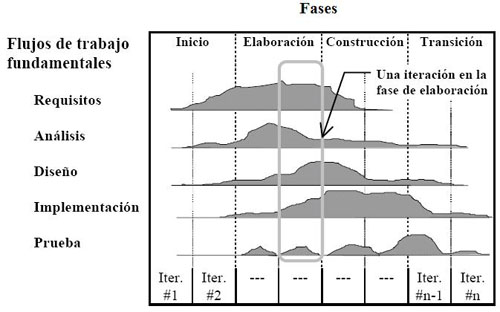
\includegraphics[
   keepaspectratio=true
]{./03_Met_Plan/01_Metodologia/diagramaProcesoUnificado.JPG}
\caption{Ciclo de vida - Proceso Unificado de Desarrollo}
\end{figure}


Cada ciclo consta de cuatro fases: \textbf{Inicio}, \textbf{Elaboración}, \textbf{Construcción} y \textbf{Transición}. Cada fase se divide en iteraciones, en las cuales se desarrolla, secuencialemte, una serie de disciplinas o flujos de trabajo: \textit{Análisis, Diseño, Implementación y Pruebas.}

En la figura podemos observar que el ciclo de vida del Proceso Unificado presenta dos dimensiones:
\begin{itemize}
	\item Un eje horizontal que representa el aspecto dinámico del proceso conforme se va desarrollando. Expresado en términos de \textit{Fases, Iteraciones e Hitos}.
	\item Un eje vertical que representa el aspecto estático del proceso mediante las disciplinas o flujos de trabajo.
\end{itemize}


\subsection{Fases}

\subsection{Fase de inicio}
Durante la fase de inicio se desarrolla una descripción del producto final y se presenta el análisis de negocio.

El objetivo de esta fase es ayudar al equipo de proyecto a decidir cuales son los verdaderos objetivos del proyecto.

\subsection{Fase de elaboración}
En esta fase se especifican la mayoría de los casos de uso del producto y se diseña la arquitectura del mismo. Se establece una firme comprensión del problema a solucionar.


\subsection{Fase de construcción}
Durante la fase de construcción se elabora el producto, de tal manera que la línea base de la arquitectura avanza hasta convertirse en el sistema completo. Al final de esta fase se obtienen todos los casos de uso implementados aunque pueden incluir defectos.


\subsection{Fase de transición}
La fase de transición hace referencia al período donde el software ya debe estar listo para ser instalado, probado y utilizado. Las iteraciones en esta fase continúan agregando características al software.

\section{Iteraciones}